%!TEX root=../oi-magistr-si.tex
\section[AOS - WS]{Webové služby. K čemu slouží? Popis a vyhledávání služeb. Technologie pro implementaci a nasazení služeb a klientů. Protokoly, kódování obsahu. Top-down a bottom-up design}

\subsection{Webové služby}
W3C definice - SW systém designovaný k vzájemné \textit{machine-to-machine} spolupráci přes internet, který má API přístupné přes \textbf{HTTP}, rozhraní je popsáno v strojové čitelném formátu (\textbf{WSDL}) a interakce s WS je pomocí \textbf{SOAP}  zpráv (HTTP + XML).

\paragraph{RPC Web Service} RPC webové služby představují volání vzdálené funkce. Metoda je popsána jako operace ve WSDL. Parametry metody i odpověď jsou posílány jako XML zabalené v SOAP. Vetšinou je implementováno jako mapování služby přímo na jazykově specifické volání funkce. Není tedy loosely coupled.

\paragraph{SOA Web Service} Webové služby se také používají k implementaci SOA, kde je základní jednotkou komunikace zpráva, nikoli operace. Tato skutečnost je často označována jako „message-oriented“ služba.
Na rozdíl od RPC webových služeb jsou SOA webové služby loose coupled, jelikož jsou zaměřeny na kontrakt poskytnutý WSDL, ne na implementační detaily.

\paragraph{RESTfull Web services} RESTfull webové služby jsou speciální podmnožinou webových služeb, které mají sadu předem definovaných operací. Tyto předem definované operace jsou přímo operace převzaté z protokolu HTTP, jedná se tedy o operace GET, POST, HEAD, atd. Každá z operací má vymezené svoje postavení vůči zdroji, který je identifikován pomocí URL. Následující tabulka shrnuje použití jednotlivých HTTP funkcí z pohledu REST služeb.

Využití metod ve správném významu je zcela klíčové pro čisté REST služby. Existuje mnoho reálných implementací webových služeb, kde je právě tento princip porušen.


\subsection{Vyhledávání služeb - UDDI registr}
UDDI (The Universal Description, Discovery and Integration Service) poskytuje mechanismus, přes který mohou klienti dynamicky hledat požadované webové služby. Tímto způsobem by aplikace měly být schopny se kontaktovat na služby poskytované externími partnery. Registr UDDI má dva druhy klientů: ty, kteří chtějí nějakou službu poskytovat a ty, kteří chtějí službu využívat.

\begin{itemize}[itemsep=0px]
\item platformně nezávislý XML-based registr služeb
\item mechanismus pro hledání WS
\item registry:
\begin{itemize}[itemsep=0px]
\item white pages - adresy, kontakty, identifikátory
\item yellow pages - kategorizace servis založena na standartních taxonomiích
\item green pages - technický popis servis (jak k ní přistoupit atd.)
\end{itemize}
\end{itemize}

\begin{figure}[h!]
\centering
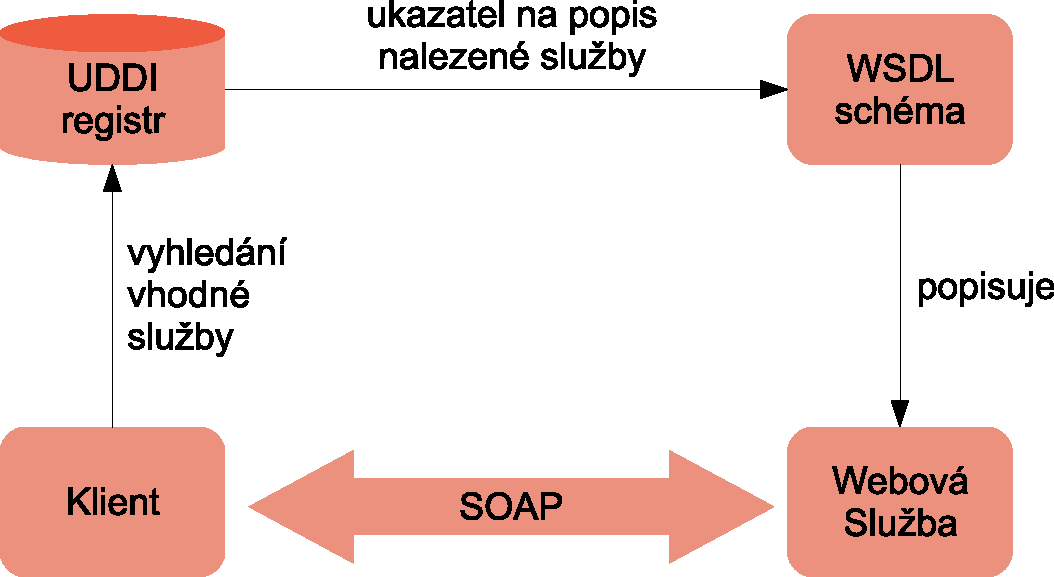
\includegraphics[width=80mm]{10/images/uddi}
\end{figure}

\subsection{Technologie a protokoly}
\subsubsection*{RPC (Remote Procedure Call)}
\begin{itemize}[itemsep=0px]
\item technologie dovolující programu vykonat proceduru (zavolat službu), která může být uložena na jiném místě než je umístěn sám volající program
\item klient/server model
\item synchronní volání klienta - je blokován dokud server neodpoví
\item může nastat chyba v případě chyby sítě
% \item obrázek vlevo
\end{itemize}
\subsubsection*{CORBA (Common Object Request Broker Architecture)}
\begin{itemize}[itemsep=0px]
\item standard, který umožňuje komunikaci mezi různými platformami a jazyky
\item jazykově, technologicky a platformě nezávislý
\item specifikace zahrnuje: silné typování, výjimky, síťový protokol
\item CORBA Interface Definition Language
\item transakce, security, marshalling
% \item obrázek vpravo
\end{itemize}
\subsubsection*{DCOM (Distributed Component Object Model)}
\begin{itemize}[itemsep=0px]
\item microsoftí CORBA (konkurent)
\item garbage collecting - uvolnění referencí držených klientem (např. při ztrátě spojení)
\end{itemize}
\subsubsection*{WSDL (Web Services Description Language)}
\begin{itemize}[itemsep=0px]
\item XML-based jazyk, který poskytuje popis (rozhraní) servici
\item služby jsou definovány jako množina síťových endpointů (portů s adresami a
bindováním)
\item popisuje veřejný interface servici
\end{itemize}
\subsubsection*{REST (Representational State Transfer)}
\begin{itemize}[itemsep=0px]
\item architektonický styl nebo množina principů pro tvorbu WS
\item klienti/servery
\item klient se dotáže - server zpracuje požadavek a vrátí odezvu
\item původně popsán pro HTTP (ale není na něj omezen)
\item vlastnosti:
\begin{itemize}[itemsep=0px]
\item stateless
\item cacheable
\item layered system
\item code on demand (opt)
\item uniform interface
\end{itemize}
\end{itemize}
\subsubsection*{SOAP (Simple Object Access Protokol)}
Jelikož veškerá komunikace mezi službami je založená na posílání zpráv, musely být zavedeny takové standardy, aby služby mezi sebou komunikovaly jednotným způsobem. Takovýmto standardem se stal SOAP. SOAP je protokol umožňující spotřebiteli služeb komunikovat s jejich poskytovatelem. Tento protokol je nezávislý na typu sítě, podporuje zprávy ve formátu XML a v současné době je ve specifikaci 1.2 od organizace W3C.

\begin{itemize}[itemsep=0px]
\item specifikace pro výměnu strukturovaných informací pomocí webových služeb
\item SOAP je nezávislý na transportních protokolech. HTTP je jen jedním z podporovaných.
\item postaveno na WSDL a UDDI
\item navrženo jako object-access protokol
\end{itemize}

\paragraph{Struktura zprávy v SOAP}
Každá zpráva dodržující podmínky kladené SOAP je v podstatě balíček (obálka, angl. envelope). Tento balíček obsahuje hlavičku (angl. head) a tělo (angl. body). Hlavička se skládá z několika bloků, které obsahují metainformace. Hlavička je nepovinná (tzn. může být vynechána). Metainformace v sobě ukrývají část komunikační logiky a obecně umožňují zavádět nová rozšíření. Typicky hlavička obsahuje nutné informace pro všechny služby, které mohou zprávu obdržet. Cílová služba potom na základě těchto informací rozhodne o způsobu zpracování zprávy. Tělo obsahuje samotná data (ve formátu XML). Tělo může také obsahovat sekci pro
chyby (angl. faults), která obsahuje logiku pro zpracování výjimek. Většinou jsou v této části uloženy jednoduché zprávy, které slouží k odeslání informací o chybě při výskytu výjimky. SOAP zahrnuje také prostředky pro posílání dat, která jsou těžko popsatelná pomocí XML (binární data, např. obrázky). Takováto data se posílají jako přílohy (angl. attachments).

\subsection{Kódování obsahu}
Posílaný obsah je potřeba nějakým způsobem reprezentovat. Požadavky jsou aby \textbf{reprezentace} (zakódování) byla lidsky \textbf{čitelná}, \textbf{neukecaná} (binary efficient - chceme posílat co nejmenší obsah), platformně \textbf{nezávislá} a \textbf{standardizovaná}.

\begin{itemize}[itemsep=0px]
\item XML - příliš ukecané
\item JSON - používané
\item YAML
\item buffers by Google
\end{itemize}

\subsection{Bottom-up design}
Nejdříve je naimplementována služba v konkrétním jazyce, následně je vygenerováno WSDL. Považováno za jednodušší návrh. Riziko vzniku závislosti na programovacím jazyku či platformě.

\subsection{Top-down design}
Nejdřive je napsán WSDL dokument (koresponduje s SOA modelem), následně je z něj vygenerován kód. Považováno za obtížnější. výsledkem je ale čistší design.
